%%%%%%%%%%%%%%%%%%%%%%%%%%%%%%%%%%%%%
%%%%%%%%%%%%%%%%%%%%%%%%%%%%%%%%%%%%%
%
%   Hi, All 
%
%   Arun Xavier, VAST Thrissur
%
%   for more  Visit my Page - http://arunxeee.blogspot.in/
%
%%%%%%%%%%%%%%%%%%%%%%%%%%%%%%%%%%%%
%%%%%%%%%%%%%%%%%%%%%%%%%%%%%%%%%%%%
%%%%%%%%%%%%%%%%%%%%%%%%%%%%%%%%%%%%%
%%%%%%%%%%%%%%%%%%%%%%%%%%%%%%%%%%%%%
%
%   Hi, All
%   Arun Xavier, VAST Thrissur
%
%   for more  Visit my Page - http://arunxeee.blogspot.in/
%
%%%%%%%%%%%%%%%%%%%%%%%%%%%%%%%%%%%%
%%%%%%%%%%%%%%%%%%%%%%%%%%%%%%%%%%%%
%
%
%
%******************************************************
%

%%
\documentclass[12 pt, oneside]{book}
\usepackage{graphicx, fancyhdr, amsmath, times,  enumerate,geometry,makeidx,setspace,nomencl,eso-pic,xcolor,lipsum,calc,pst-node,tikz,fancybox,background,caption,subcaption,amsfonts}



\usetikzlibrary{calc}
\SetBgScale{1}
\SetBgAngle{0}
\SetBgColor{brown}
\SetBgOpacity{1}
%%
\geometry{verbose,a4paper,tmargin=1 in,bmargin=1in,lmargin=1.5 in,rmargin=.9 in}
%%%%%%%%%%%%%%%%%%%%%%%%%%%%%%%

\makeindex

%%
\usepackage[final]{pdfpages}
%%
%\setlength{\oddsidemargin}{2 cm}
%%
\newcommand{\VAtitle}[1]%
{\def\vtitle{#1}}%
\newcommand{\VAauthor}[1]%
{\def\vauthor{#1}}%
\newcommand{\VAadmissionyear}[1]%
{\def\vadmissionyear{#1}}%
\newcommand{\VAacademicyear}[1]%
{\def\vacademicyear{#1}}%
\newcommand{\VAregisternumber}[1]%
{\def\vregisternumber{#1}}%
\newcommand{\VAprincipal}[1]%
{\def\vprincipal{#1}}%
\newcommand{\VAguide}[1]%
{\def\vguide{#1}}%
\newcommand{\VAguidedg}[1]%
{\def\vguidedg{#1}}%
\newcommand{\VAhod}[1]%
{\def\vhod{#1}}%
\newcommand{\VAmonth}[1]%
{\def\vmonth{#1}}%
\newcommand{\VAdept}[1]%
{\def\vdept{#1}}%
\newcommand{\VAclass}[1]%
{\def\vclass{#1}}%
\newcommand{\VApaper}[1]%
{\def\vpaper{#1}}%
%%
%%
%\renewcommand\bibname{References}




\SetBgContents{}

\VApaper{SEMINAR REPORT}


\usepackage{titlesec}
\titleformat{\chapter}[display]
{\normalfont\huge\bfseries\centering}{\chaptertitlename\ \thechapter}{20pt}{\Huge}

\DeclareUnicodeCharacter{2212}{-}
\begin{document}
%%%%%%%%%%%%%%%%%%%%%%%%%%%%%%%%%%%%
%%%%%%%%%%%%%%%%%%%%%%%%%%%%%%%%%%%%
%	Edit from Below . . . 
%   In the next line, replace "ReportTitle" by 
%   the title of your seminar
%
\VAtitle{Primary Care Interventions for Dementia Using Data Mining}
%
%
%   In the next line, replace "Student" by your name. 
%   Write full name without, Mr. or Ms.
%
\VAauthor{SHOUKKIYA ASHRAF}%
%
%
\VAadmissionyear{2016}%
%
\VAacademicyear{2016-2020}%
%
%   University Examination Register Number.
%
\VAregisternumber{VAS16CS107}% 
%
%   the full name of your guide or supervisor 
%   with Mr. or Ms. or Dr. or Prof.
%

\VAprincipal{Dr.Saji C B}% 
\VAguide{Sivadasan E. T}% 
\VAguidedg{Asso. Prof}
 % Give your Guides Designation Asst. Prof., Asso. Prof.
%
%   In the next line, replace "HoD" by 
%   the full name of Head of Department 
%   with Mr. or Ms. or Dr. or Prof.
%
\VAhod{Dr.Ramani Bhai}
%
%   Enter the Sem End month like "December"
%   Type Month and Year
\VAmonth{November 2019}%
\VAdept{Computer Science}%
\VAclass{Seventh Semester B.Tech}%
%%%%%%%%%%%%%%%%%%%%%%%%%%%%%%%%%%%%%
%%%%%%%%%%%%%%%%%%%%%%%%%%%%%%%%%%%%%
%%%%%%%%%%%%%%%%%%%%%%%%%%%%%%%%%%%%%
%%%%%%%%%%%%%%%%%%%%%%%%%%%%%%%%%%%%%
%
%   Hi, All
%   Arun Xavier, VAST Thrissur
%
%   for more  Visit my Page - http://arunxeee.blogspot.in/
%
%%%%%%%%%%%%%%%%%%%%%%%%%%%%%%%%%%%%
%%%%%%%%%%%%%%%%%%%%%%%%%%%%%%%%%%%%
%
%
%
%******************************************************
%
% 
%  
\fancypagestyle{plain}{%
\fancyhf{} % clear all header and footer fields
\fancyhead[L]{{\scriptsize \vtitle}}
\fancyhead[R]{
\includegraphics[width=0.5cm]{VidyaLogo.JPG}}
%\fancyfoot[C]{\bfseries \thepage} 
\fancyfoot[L]{{\footnotesize Department of Computer Science Engg.}}
\fancyfoot[R]{\footnotesize VAST, Thalakotukara}
\fancyfoot[C]{\footnotesize \bf \thepage}%
\renewcommand{\headrulewidth}{1pt}%
\renewcommand{\footrulewidth}{1pt}%
}%
%
%
\pagestyle{empty}
%
%%%%%%%%%%%%%%%%%%%%%%%%%%%%%%%%%%%%%
%%%%%%%%%%%%%%%%%%%%%%%%%%%%%%%%%%%%%
%
%   Hi, All
%   Arun Xavier, VAST Thrissur
%
%   for more  Visit my Page - http://arunxeee.blogspot.in/
%
%%%%%%%%%%%%%%%%%%%%%%%%%%%%%%%%%%%%
%%%%%%%%%%%%%%%%%%%%%%%%%%%%%%%%%%%%
%
%******************************************************
%

\begin{spacing}{1.5}
\begin{titlepage}




\SetBgContents{

\begin{tikzpicture}[overlay,remember picture]
\draw [line width=3pt]
    ($ (current page.north west) + (3.0cm,-1.8cm) $)
    rectangle
    ($ (current page.south east) + (-1.35cm,1.8cm) $);
\draw [line width=1pt]
    ($ (current page.north west) + (3.15cm,-1.95cm) $)
    rectangle
    ($ (current page.south east) + (-1.5cm,1.95cm) $); 
\end{tikzpicture}
}

\begin{center}


{ \LARGE \rmfamily \bf \vtitle}\\[1 cm]

{ \large \rmfamily \vpaper \\ SUBMITTED IN PARTIAL FULFILLMENT OF THE \\REQUIREMENTS FOR THE AWARD OF DEGREE OF}\\[1 cm]

{ \Large \rmfamily \bf BACHELOR OF TECHNOLOGY}\\
{\large \rmfamily in}\\[.4 cm]
{ \Large \rmfamily \bf COMPUTER SCIENCE AND ENGINEERING}\\
{\large \rmfamily of}\\[.4 cm]
{ \Large \rmfamily \bf APJ Abdul Kalam Technological University}\\
{\large \rmfamily by}\\[1 cm]
{\large \rmfamily \bf \vauthor} \\
{\large \bf Univ. Reg.No. \vregisternumber} \\[2 cm]
%

%
\includegraphics[width=3.5 cm]%
{VidyaLogo.JPG}\\
\scriptsize (AN ISO 9001:2008 CERTIFIED INSTITUTION )\\[1.5 cm]

%
{\Large \bf Department of \vdept} \\
{\Large \rmfamily Vidya Academy of Science \& Technology\\[.2 cm]
\large Thalakkottukara, Thrissur - 680 501}\\
({ \bf \tt http://www.vidyaacademy.ac.in})\\[.1 cm]
{\large \rmfamily \vmonth}


\end{center}
\end{titlepage}
%
%******************************************************
%
%
\clearpage
\pagenumbering{roman}
%


%\addcontentsline{toc}{chapter}{\quad Certificate}

\begin{titlepage}
\SetBgContents{

\begin{tikzpicture}[overlay,remember picture]
\draw [line width=3pt]
    ($ (current page.north west) + (3 cm,-1.8cm) $)
    rectangle
    ($ (current page.south east) + (-1.5cm,1.8cm) $);
\draw [line width=1pt]
    ($ (current page.north west) + (3.15cm,-1.95cm) $)
    rectangle
    ($ (current page.south east) + (-1.65cm,1.95cm) $); 
\end{tikzpicture}
}


\begin{center}


{\Large \bf Department of \vdept  }\\
{\Large \bf Vidya Academy of Science \& Technology}\\
{\normalsize \bf Thalakkottukara, Thrissur - 680 501\\
({\tt http://www.vidyaacademy.ac.in})}\\[0.75cm]
%
%   Logo
%

\includegraphics[width=3.5 cm]{VidyaLogo.JPG}\\
\scriptsize (AN ISO 9001:2008 CERTIFIED INSTITUTION )\\[1 cm]
%
 \Huge  $ \mathfrak{Certificate}$\\[0.5cm]
%
\end{center}
\index{Certificate}
\index{University of Calicut}

\quad This is to certify that the seminar report titled {\bf ``\vtitle"} is a bonafide record of the work carried out by {\bf \vauthor\ } {\bf (Univ. Reg.No. \vregisternumber) } of Vidya Academy of Science \& Technology, Thalakkottukara, Thrissur - 680 501 in partial fulfillment of the requirements for the award of {\bf Degree of Bachelor of Technology} in {\bf Computer Science and  Engineering} of  {\bf APJ Abdul Kalam Technological University}, during the academic year \vacademicyear. \\[2 cm]
 
\noindent{\bf Seminar Guide/Supervisor} \hfill  {\bf Head of Department} \\[.3cm]
\noindent \vguide \hfill \vhod \\ \vguidedg\ Dept. of  CSE \hfill Prof., Dept. of CSE  



%
\end{titlepage}


%   End of Certificate
%  
%
\clearpage
\pagestyle{plain}
%

\addcontentsline{toc}{chapter}{\quad ACKNOWLEDGEMENT}
%%%%%%%%%%%%%%%%%%%%%%%%%%%%%%%%%%%%%
%%%%%%%%%%%%%%%%%%%%%%%%%%%%%%%%%%%%%
%
%   Hi, All
%   Arun Xavier, VAST Thrissur
%
%   for more  Visit my Page - http://arunxeee.blogspot.in/
%
%%%%%%%%%%%%%%%%%%%%%%%%%%%%%%%%%%%%
%%%%%%%%%%%%%%%%%%%%%%%%%%%%%%%%%%%%
%
%
%
%******************************************************
%
%
\chapter*{Acknowledgement}
%


\par
\hspace{0.9cm}I wish to record my indebtedness and thankfulness 
to all those who helped me prepare this report titled ``{\bf \vtitle\ }''  and present it in a satisfactory way.

\vspace {.2cm}
\par
\hspace{.35cm}First and foremost I thank God Almighty for His providence and for being the guiding light throughout the seminar.

\vspace{0.2cm}
\par
\hspace{0.35cm}I would like to thank my guide {\bf \vguide, } \vguidedg\ of \vdept\  Dept. for providing critical inputs in the preparation of this report. I also thank all other faculty members in our department for their guidance.


\vspace{.2cm}
\par 
\hspace{.35cm}I am thankful to {\bf \vhod}, 
Head of \vdept\  Department, and our Principal {\bf \vprincipal}, for their sole co-operation.



\vspace{0.2cm}
\par
\hspace{0.35cm}Finally, I would like to extend my sincere gratitude to friends who have always been helpful, in preparing and presenting the report and in the discussion following the presentation.

\begin{flushright}
\vauthor\\
Reg. No. \vregisternumber\\
\vclass\  ( \vadmissionyear\  Admissions)\\
Vidya Academy of Science \& Technology\\
Thrissur - 680 501.
\end{flushright}

\vmonth\ 


%
\clearpage
%
				% Dont Edit . . 
%%%%%%%%%%%%%%%%%%%%%%%%%%%%%%%%%%%%%
%%%%%%%%%%%%%%%%%%%%%%%%%%%%%%%%%%%%%
%
%
\chapter*{Abstract}
\addcontentsline{toc}{chapter}{\quad ABSTRACT}
Dementia and cognitive impairment associated with aging are a major medical and social concern. Elderly people constitute a significant percentage of the population all over the world. Patient Central Bureau of General Mobilization and Statistics (2013) reported that elderly represent 6.9\% of the Egyptian population, it is estimated that the number of elderly people will be replicated in 2030. Eight percent (8\%) of elders aged between 65 \& 74, also about 50\% aged over 80 suffer from the cognitive disease or dementia. The core of this study is to use intelligent techniques to fulfill specific needs of cognitive deficits patients and assess interaction changes based on patient’s behavior in various disease stages. The aim  is to provide a usable and effective help for elderly. The proposed idea will be divided into three main phases, evaluation phase, data mining phase and assistance phase. Patient proceeds in the three stages by behavior analysis and feedback to provide interactive evaluation and assistance for him/her.Data Mining phase consists of discovering a certain pattern in huge datasets.Here,the mined information not only help understand the physiological and pathological nature of dementia, but also assist physicians in prognostic risk assessments and developing the best treatment method.
%%%%%%%%%%%%%%%%%%%%%%%%%%%%%%%%%%%%
%%%%%%%%%%%%%%%%%%%%%%%%%%%%%%%%%%%%
\tableofcontents
\addcontentsline{toc}{chapter}{\quad  LIST OF FIGURES}
\listoffigures
\addcontentsline{toc}{chapter}{\quad  LIST OF  TABLES}
\listoftables
% For adding List of symbols or abbreviations
%\addcontentsline{toc}{chapter}{\quad  LIST OF SYMBOLS AND ABBREVIATIONS}
%%%%%%%%%%%%%%%%%%%%%%%%%%%%%%%%%%%%%%
%%%%%%%%%%%%%%%%%%%%%%%%%%%%%%%%%%%%%
%
%   Hi, All
%   Arun Xavier, VAST Thrissur
%
%   for more  Visit my Page - http://arunxeee.blogspot.in/
%
%%%%%%%%%%%%%%%%%%%%%%%%%%%%%%%%%%%%
%%%%%%%%%%%%%%%%%%%%%%%%%%%%%%%%%%%%
%
%
%
%******************************************************
%



\chapter*{List of Symbols and Abbreviations}




\begin{tabbing}



\hspace{1cm}\= {$ \bf VAST  $}\quad\= Vidya Academy of Science and Technology\\[5pt]

\> {$ \bf A_i  $} \> Area of the $i^{th}$ component\\[5pt]

\> {$ \bf DC $} \>   Direct current electricity\\[5pt]

\> {$ \bf DSO  $} \> Digital Storage Oscilloscope\\[5pt]

\> {$ \bf FBI  $} \> Full Bridge Inverter




\end{tabbing}
%\mainmatter			
%%%%%%%%%%%%%%%%%%%%%%%%%%%%%%%%%%%%
%%%%%%%%%%%%%%%%%%%%%%%%%%%%%%%%%%%%
%   The main contents of the paper begin here. 
%   In the following replace with 
%   the title of the first chapter of your paper.
%
\chapter{INTRODUCTION}

{\em Dementia is a broad category of brain diseases that cause a long-term and often gradual decrease in the ability to think and remember that is severe enough to affect a person's daily functioning. }

\section{General}    % For giving Section  eg: 1.1

Dementia is a degenerative brain disease that affects cognitive abilities of patients in general and the elderly, in specific . This disease has many forms such as Alzheimer diseases (AD), Vascular dementia, Dementia with Lewy bodies (DLB), Mixed dementia, Frontal temporal lobar degeneration (FTLD). That affects cognitive abilities of patients such as memory, language,communication skills and all daily life activates .\\
Human-Computer interaction can be defined as a powerful tool used to make technologies more usable, simple and adaptive for everybody and especially with disabilities. Human-Computer Interaction (HCI) points out the design and implementation of computer based systems that different types of people interact with, including embedded systems in all kinds of devices, and desktop systems, as well . HCI is heedful with the following:\\
1. The user interface between computer and user for designing of the menus and screens,\\
2. The dialectics for building the functionality into the system.\\
3. The sequent of using the system over time and its impacts on the society, group, and individual.\\
 
%%%%%%%%%%%%%%%%%%%%%%%%%%%%%%%%%%%
%		Before using image put the jpg image file in the folder. 
%		Here   1.jpg   is the file name
%%%%%%%%%%%%%%%%%%%%%%%%%%%%%%%%%%%
%\begin{figure}[h]
	%\begin{center}
		%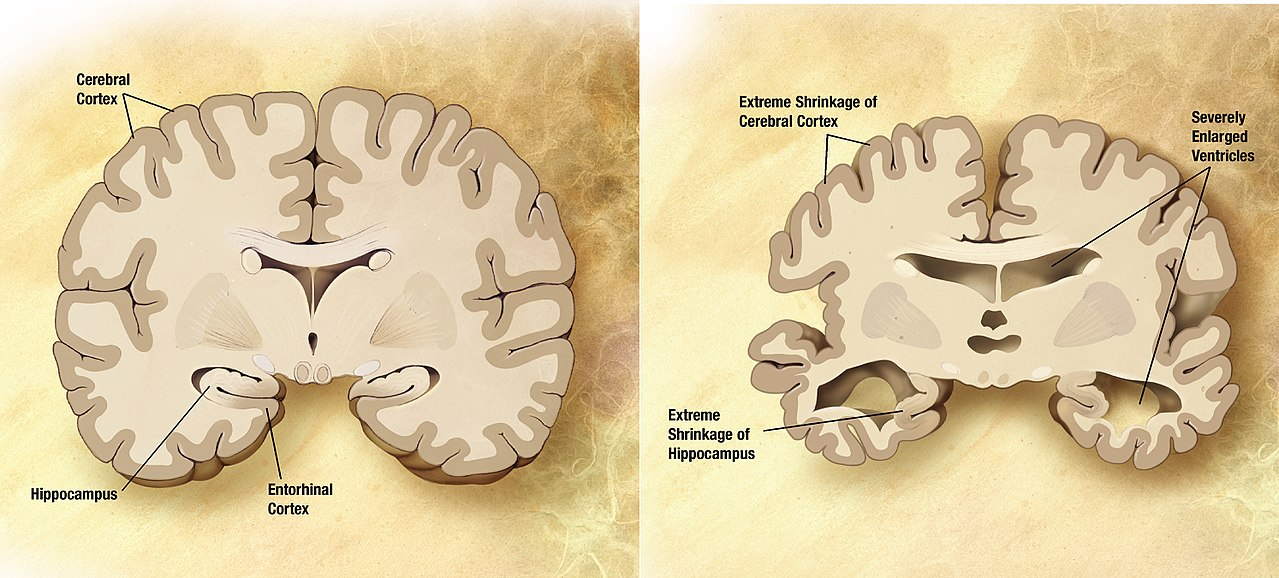
\includegraphics[width =5 cm]{1.jpg}
		%\caption{Resonance based inertial Electromagnetic Microgenerator}
		%\label{ab}
	%\end{center}
%\end{figure}

%\begin{figure}[h]
%\begin{center}
%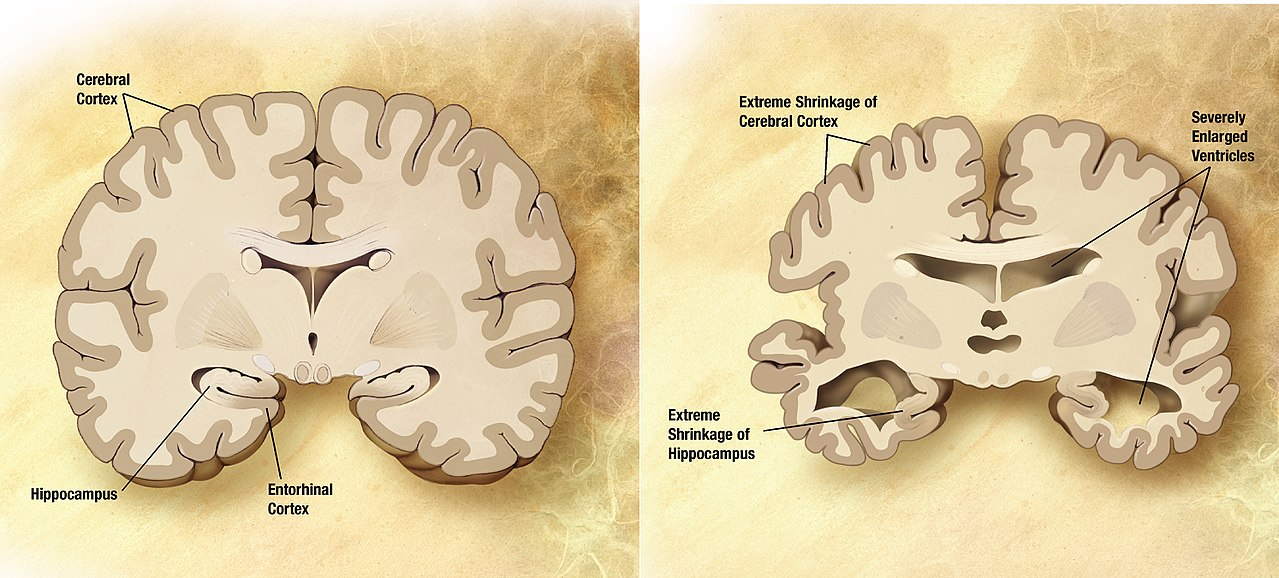
\includegraphics[width =5 cm]{1.jpg}
%\caption{Resonance based inertial Electromagnetic Microgenerator}
%\label{a}
%\end{center}
%\end{figure}



 \section{OBJECTIVE OF THE WORK}     % You can add any sections like that . . 

The work focussed on assistive technologies that based on HCI models are facilitators that can be utilized to improve the quality of life for patients, disabled, and elderly. It can assist human in a more natural way to interact with his environment. 

\section{OUTLINE OF REPORT}

First Chapter contains introduction to Primary Care Interventions for Dementia Using Data Mining. Second chapter contains case study of Dementia. Third chapter is  Human-Computer Interaction. Fourth chapter is  about Data mining and the fifth chapter contains an introduction to natural language processing.The sixth chapter contains conclusion.



\chapter{ CASE STUDY - DEMENTIA}			%Difft Sections in IEEE Paper

{\em There is no known cure for dementia. The symptoms of dementia vary across types and stages of the diagnosis.The most common affected areas include memory, visual-spatial, language, attention and problem solving. }

\section{SIGNS AND SYMPTOMS}

 Most types of dementia are slow and progressive. By the time the person shows signs of the disorder, the process in the brain has been happening for a long time. It is possible for a patient to have two types of dementia at the same time. About 10\% of people with dementia have what is known as mixed dementia, which is usually a combination of Alzheimer's disease and another type of dementia such as frontotemporal dementia or vascular dementia [1].Neuropsychiatric symptoms that may be present are termed Behavioural and psychological symptoms of dementia (BPSD) and these can include:
\begin{itemize}
  \item Balance problems
  \item Tremor
\item Speech and language difficulty
\item Trouble eating or swallowing
\item  Memory distortions (believing that a memory has already happened when it has not, thinking an old memory is a new one, combining two memories, or confusing the people in a memory)
\item Wandering or restlessness
\item Perception and visual problems
\item Behavioral and psychological symptoms of dementia almost always occur in all types of dementia and may manifest as:[2][3]
\item Agitation
\item Depression
\item Anxiety
\item Abnormal motor behavior
\item Elated mood


\end{itemize}
\begin{figure}[h]
	\begin{center}
		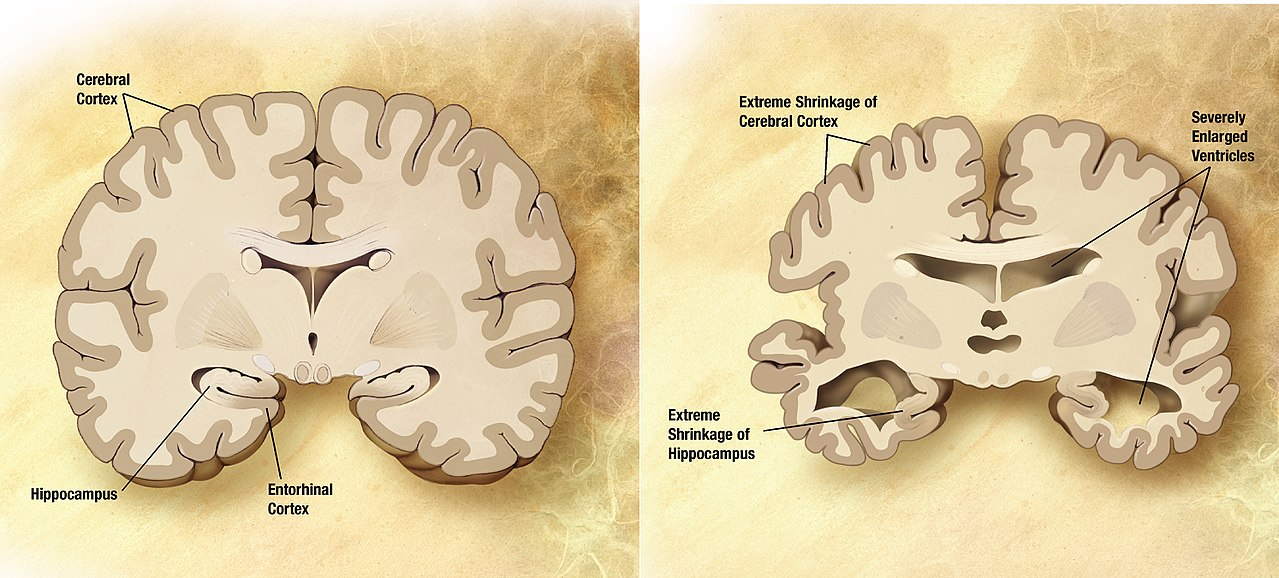
\includegraphics[width =10cm]{1.jpg}
		\caption{Comparison of a normal aged brain (left) and the brain of a person with Alzheimer's disease (right)}
		\label{ab}
	\end{center}
\end{figure}


When people with dementia are put in circumstances beyond their abilities, there may be a sudden change to crying or anger (a "catastrophic reaction").Psychosis (often delusions of persecution) and agitation/aggression also often accompany dementia.



\section{ STAGES OF DEMENTIA}

It starts with little symptoms and gradually increases.When people with dementia are put in circumstances beyond their abilities, there may be a sudden change to crying or anger (a "catastrophic reaction"). These are the main stages of dementia diseases like Alzheimer.
\\ Dementia diseases don’t appear all at once, but they start with little symptoms and gradually increase. The speed of symptoms increasing inversely proportional to brain actives like memory training, short and long activities for attention and concentration which help in increasing cognitive abilities. We aim in this research to stand against and delay degenerative brain and memory loss with cognitive brain activities. Cognitive deficits such as Alzheimer and dementia are the most common diseases that affect cognitive abilities for elders. As these diseases advances, more symptoms appear which negatively affect memory, language, and communication
skill. It also causes depression and sleep disorders. Until now there is no cure for cognitive deficits that lead to functions loss and ultimately death. Current solutions only help in living with symptoms and decrease the speed of function loss . 

\begin{figure}[h]
\begin{center}
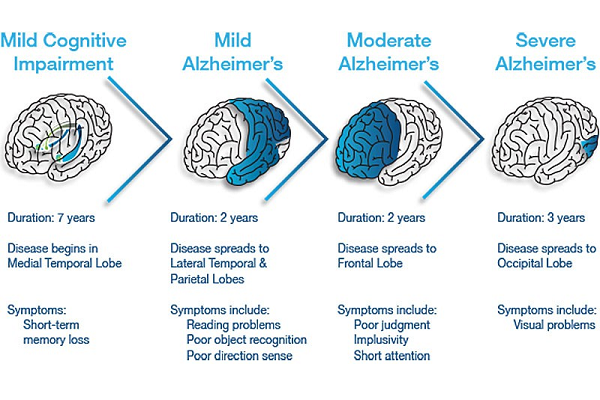
\includegraphics[width = 13 cm]{5.PNG}
\caption{Distinct stages of Dementia}
\end{center}
\end{figure}


In the first stages of dementia, the signs and symptoms of the disorder may be subtle. Often, the early signs of dementia only become apparent when looking back in time. The earliest stage of dementia is called mild cognitive impairment (MCI). 70\% of those diagnosed with MCI progress to dementia at some point.\\
As dementia progresses, the symptoms first experienced in the early stages of the dementia generally worsen. The rate of decline is different for each person. A person with moderate dementia scores between 6–17 on the MMSE.\\
People with late-stage dementia typically turn increasingly inward and need assistance with most or all of their personal care. Persons with dementia in the late stages usually need 24-hour supervision to ensure personal safety, as well as to ensure that basic needs are being met. If left unsupervised, a person with late-stage dementia may wander or fall, may not recognize common dangers around them such as a hot stove, may not realize that they need to use the bathroom or become unable to control their bladder or bowels (incontinent)[4]\\
Changes in eating frequently occur. Caregivers of people with late-stage dementia often provide pureed diets, thickened liquids, and assistance in eating, to prolong their lives, to cause them to gain weight, to reduce the risk of choking, and to make feeding the person easier.The person's appetite may decline to the point that the person does not want to eat at all. They may not want to get out of bed, or may need complete assistance doing so. Commonly, the person no longer recognizes familiar people. They may have significant changes in sleeping habits or have trouble sleeping at all.
\begin{figure}[h]
\begin{center}
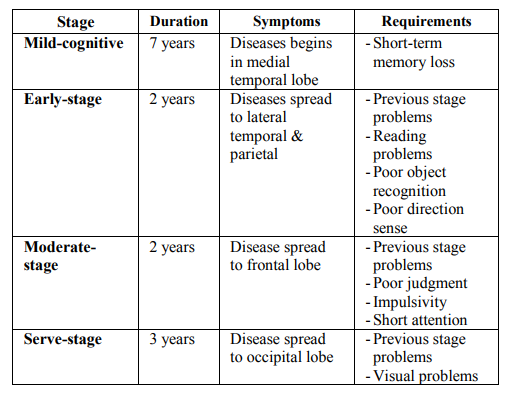
\includegraphics[width = 13 cm]{3.PNG}
\end{center}
\end{figure}
\begin{table}[h]
\caption{Stages of Dementia}
\end{table}


\section{DIAGNOSIS}

Diagnosis may be aided by brain scanning techniques. In many cases, the diagnosis cannot be absolutely sure except with a brain biopsy, but this is very rarely recommended (though it can be performed at autopsy). In those who are getting older, general screening for cognitive impairment using cognitive testing or early diagnosis of dementia has not been shown to improve outcomes.\\
Normally, symptoms must be present for at least six months to support a diagnosis. Cognitive dysfunction of shorter duration is called delirium. Delirium can be easily confused with dementia due to similar symptoms. Delirium is characterized by a sudden onset, fluctuating course, a short duration (often lasting from hours to weeks), and is primarily related to a somatic (or medical) disturbance. In comparison, dementia has typically a long, slow onset (except in the cases of a stroke or trauma), slow decline of mental functioning, as well as a longer duration (from months to years).Changes in thinking, hearing and vision are associated with normal ageing and can cause problems when diagnosing dementia due to the similarities.\\A CT scan or magnetic resonance imaging (MRI scan) is commonly performed, although these tests do not pick up diffuse metabolic changes associated with dementia in a person that shows no gross neurological problems (such as paralysis or weakness) on neurological exam.[citation needed] CT or MRI may suggest normal pressure hydrocephalus, a potentially reversible cause of dementia, and can yield information relevant to other types of dementia, such as infarction (stroke) that would point at a vascular type of dementia.The functional neuroimaging modalities of SPECT and PET are more useful in assessing long-standing cognitive dysfunction, since they have shown similar ability to diagnose dementia as a clinical exam and cognitive testing.The ability of SPECT to differentiate the vascular cause (i.e., multi-infarct dementia) from Alzheimer's disease dementias, appears superior to differentiation by clinical exam.





\section{ MANAGEMENT}

There is some evidence that educating and providing support for the person with dementia, as well as caregivers and family members, improves outcomes. There is low quality evidence that regular (at least five sessions of) music therapy may help residents in institutions. It may reduce depressive symptoms and improve overall behaviour. There may also be a beneficial effect on emotional well-being and quality of life, as well as anxiety reduction. Exercise programs are beneficial with respect to activities of daily living and potentially improve dementia and these can include:
\begin{itemize}
  \item Psychological therapies
  \item Medications
\item Diet
\item Alternative medicine
\item Palliative care
\end{itemize}
All the above mentioned are not excatly sure about removig dementia perfectly.It may help to get some sort of relief.Although persistent pain in the person with dementia is difficult to communicate, diagnose, and treat, failure to address persistent pain has profound functional, psychosocial, and quality of life implications for this vulnerable population. Health professionals often lack the skills and usually lack the time needed to recognize, accurately assess, and adequately monitor pain in people with dementia. Family members and friends can make a valuable contribution to the care of a person with dementia by learning to recognize and assess their pain. Educational resources (such as the Understand Pain and Dementia tutorial) and observational assessment tools are available.
Among otherwise healthy older people, computerized cognitive training may improve memory.\\ However it is not known if it prevents dementia.Educational resources (such as the Understand Pain and Dementia tutorial) and observational assessment tools are available.\\
Dementia impacts not only the individuals with dementia, but also their carers and the wider society. Among people aged 60 years and over, dementia is ranked the 9th most burdensome condition according to the 2010 Global Burden of Disease (GBD) estimates.The global costs of dementia is around US  \textdollar 818 billion in 2015, a 35.4\% increase from US \textdollar 604 billion in 2010.\\There are some brief tests (5–15 minutes) that have reasonable reliability to screen for dementia. While many tests have been studied,presently the mini mental state examination (MMSE) is the best studied and most commonly used. The MMSE is a useful tool for helping to diagnose dementia if the results are interpreted along with an assessment of a person's personality, their ability to perform activities of daily living, and their behaviour.Other cognitive tests include the abbreviated mental test score (AMTS), the, Modified Mini-Mental State Examination (3MS).Another approach to screening for dementia is to ask an informant (relative or other supporter) to fill out a questionnaire about the person's everyday cognitive functioning. Informant questionnaires provide complementary information to brief cognitive tests. Probably the best known questionnaire of this sort is the Informant Questionnaire on Cognitive Decline in the Elderly (IQCODE).



\chapter{HUMAN COMPUTER INTERACTION}


{\em As accurate and portable brain imaging technologies become more mainstream, the nature of how we interact with computers will change completely and forever. . }

\section{INTERACTION DESIGN}

HCI in assistive technology for special diseases (disabled, elderly) aims to understand and facilitate the needs of patients and their communities (caregivers, doctors, patients). Complete HCI system for Alzheimer’s patient (AD) developed by D. Mandiliotis et al. which make an integrated system that fulfill patient’s needs in adaptive way, system provide facilities to caregivers and doctors to monitor
patient and deal with his needs (symbio music, symbio games, symbio organizer... etc.).\\ Authors of [5] provide prototype for smart environment for Alzheimer’s patient this project aims to depend on monitor patient and immediately help when error has been happened by sending text message to caregivers, this home prototype proposed built-in sensors for oven, refrigerator, sink to reduce risks and allow caregivers to monitor and follow patient actions, authors. This paper demonstrates, in theory, how HCI can be achieved in a smart environment for Alzheimer patients. Others provide multimedia story include (images, videos, music) which allow patient to interact with multimedia, this interaction adaptive dynamically according to the state of the diseases, it will help in the mid stage of cognitive deficits.\\Some studies try to interact with patients according to sensors, [6] try to extract emotions in three levels arousal valence and dominance dimensions VAD levels developed HCI system to understand and classify human emotions through VAD levels, physiological features used from DEAP dataset to analysis and extract features for emotional patterns. Extreme machine learning (ELM) used to predict emotions. Others (as shown in Fig. 2.) depend on speech and gesture as input for developing HCI System, gesture input is provided through a computer mouse (instead of a pen), speech recognition made using the open source software Pocket Sphinx. Screen recording and camera recording used as inputs datasets another type of interaction by hand gesture .\\

\begin{figure}[h]
	\begin{center}
		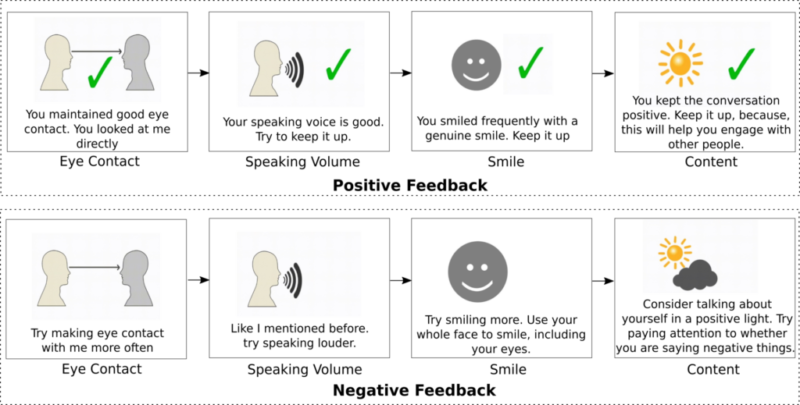
\includegraphics[width =15.5cm]{4.PNG}
		\caption{HCI -Example}
		\label{ab}
	\end{center}
\end{figure}
Healthcare industry nowadays produces big dataset about patients, disease recognition and diagnosis etc. The massive amount of data is the core of analyzing and extracting knowledge that helps in efficient decision making and cost saving. Healthcare application depends
on data mining in diagnosis, treatment and enhancing healthcare resource management etc. Using data mining and machine learning in health care would save various manual process that leads to improving patient care, data mining provides several types of processes that extract valuable information that help doctors and caregivers in taking the right decision in patient diagnosis and treatment. Machine learning in healthcare recently made huge improvements, Google developed machine learning algorithm that made diagnosis cancerous tumors based on mammograms.\\It also reported high results in skin cancer using deep neural network . Diabetic retinopathy in retinal images also diagnosed using deep machine learning algorithm . Ilayaraja et al [15] proposed data mining technique to predict the patient under risk based on some chosen features and the level of risk. This method was applied over 1000 record of heart disease patient who suffer from several heart diseases it depends on, discarding the unnecessary item set which does not satisfy the support value, this method increases efficiency
and save execution time.

\section{PHASES}
HCI points out the design and implementation of computer-based systems that  different types of people interact with. Various kinds of data are needed to simulate human- computer interactions for elderly. These data could be structured or unstructured.One of the main contributions of our research is to enhance prediction of emotion and needs of the patient based on data mining. Assistive technologies that based on HCI models are facilitators that can be utilized to improve the quality of life for patients, disabled, and elderly.  It can assist human in a more natural way to interact with his environment. Proposed framework will be divided into three main phases :\\
\begin{itemize}
  \item  Evaluation phases and Acronyms 
  \item  Data mining phase 
\item  Assistance phase

\end{itemize}
First phase is the user interface between computer and user for designing of the menus and screens and the second phase is The dialectics for building the functionality into the system. And in the  third phase contains  the sequence of using the system over time and its impacts on the society, group, and individual.System provide facilities to caregivers and doctors to  monitor patient and deal  with his needs symbio music,symbio games.
\begin{figure}[h]
	\begin{center}
		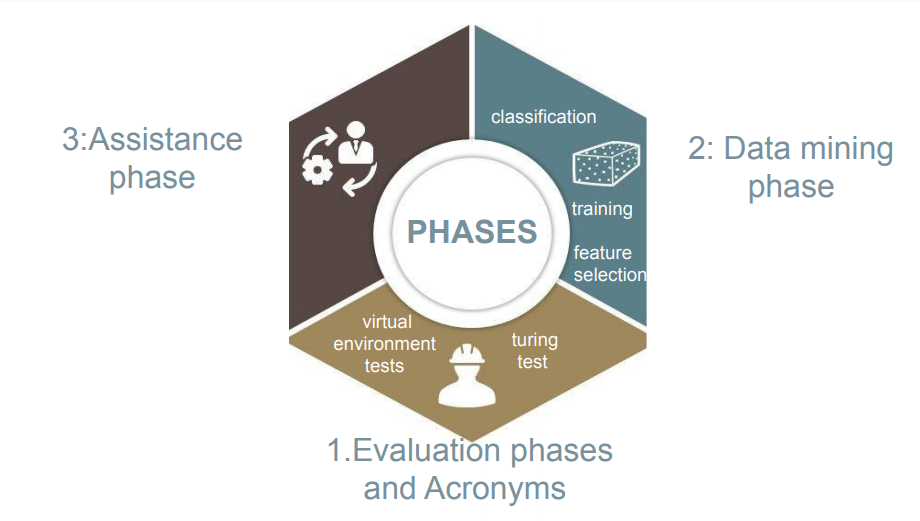
\includegraphics[width =15.5cm]{2.PNG}
		\caption{HCI - Phases}
		\label{ab}
	\end{center}
\end{figure}
\subsection {Phase 1: Evaluation phases and Acronyms}
This phase will focus on the evaluation of cognitive abilities using games and tests that evaluate short-term memory, attention, and concentration, the proposed test will focus in the evaluation of memory functions which related to recent events and conversations.
Proposed cognitive evaluation test based on turning test and virtual environment tests. This stage will be considered as an input to the third stage. System in the third stage will vary and dynamically change according to cognitive abilities.
\subsection{Phase 2: Data mining phase}
In this phase, the system will try to capture data from patient sensors and analyzeit in the real time with the clinical and the in a middle data mining layer. Physiological and vital data will be analyzed, and key features will be extracted using feature selection techniques, then training and on time classification. This stage has a great importance in understanding and developing of usable and accessible HCI interface that will assist in improving cognitive abilities of the patient.
\subsection{Phase 3: Assistance phase }
This phase is the most important phase of proposed system.The sequence of using the system over time and its impacts on the society, group, and individual contains here. It provides thefollowing possibilities:
\begin{itemize}
  \item  Use data mining from the previous step to predict patient needs.
  \item Provide mental activities to develop awareness and recognition.
\item  Make periodically assessment to the patient
\item Provide feedback and automatically adapt system according to patient status. 


\end{itemize}
Human–computer interaction (HCI) researches the design and use of computer technology, focused on the interfaces between people (users) and computers. Researchers in the field of HCI both observe the ways in which humans interact with computers and design technologies that let humans interact with computers in novel ways. As a field of research, human–computer interaction is situated at the intersection of computer science, behavioural sciences, design, media studies, and several other fields of study. Poorly designed human-machine interfaces can lead to many unexpected problems. A classic example is the Three Mile Island accident, a nuclear meltdown accident, where investigations concluded that the design of the human-machine interface was at least partly responsible for the disaster. Similarly, accidents in aviation have resulted from manufacturers' decisions to use non-standard flight instrument or throttle quadrant layouts: even though the new designs were proposed to be superior in basic human-machine interaction, pilots had already ingrained the "standard" layout and thus the conceptually good idea actually had undesirable results.\\A number of diverse methodologies outlining techniques for human–computer interaction design have emerged since the rise of the field in the 1980s. Most design methodologies stem from a model for how users, designers, and technical systems interact. Early methodologies, for example, treated users' cognitive processes as predictable and quantifiable and encouraged design practitioners to look to cognitive science results in areas such as memory and attention when designing user interfaces. Modern models tend to focus on a constant feedback and conversation between users, designers, and engineers and push for technical systems to be wrapped around the types of experiences users want to have, rather than wrapping user experience around a completed system.

\chapter{INTRODUCTION TO NATURAL LANGUAGE PROCESSING}
{\em Nowadays, it is used to power search engines, filter spam and to obtain analytics in a fast and scalable manner. Researchers are even able to boast of near human level perfection in many of these tasks, the most prominent being machine translation. With the surplus of tools and technologies dedicated to NLP, it’s so easy to get started.. }

\section{History}
The history of natural language processing (NLP) generally started in the 1950s, although work can be found from earlier periods. In 1950, Alan Turing published an article titled "Computing Machinery and Intelligence" which proposed what is now called the Turing test as a criterion of intelligence.Some notably successful natural language processing systems developed in the 1960s were SHRDLU, a natural language system working in restricted "blocks worlds" with restricted vocabularies, and ELIZA, a simulation of a Rogerian psychotherapist, written by Joseph Weizenbaum between 1964 and 1966. Using almost no information about human thought or emotion, ELIZA sometimes provided a startlingly human-like interaction. When the "patient" exceeded the very small knowledge base, ELIZA might provide a generic response, for example, responding to "My head hurts" with "Why do you say your head hurts?".\\
In the 2010s, representation learning and deep neural network-style machine learning methods became widespread in natural language processing, due in part to a flurry of results showing that such techniques can achieve state-of-the-art results in many natural language tasks, for example in language modeling, parsing,[7] and many others. Popular techniques include the use of word embeddings to capture semantic properties of words, and an increase in end-to-end learning of a higher-level task (e.g., question answering) instead of relying on a pipeline of separate intermediate tasks (e.g., part-of-speech tagging and dependency parsing). In some areas, this shift has entailed substantial changes in how NLP systems are designed, such that deep neural network-based approaches may be viewed as a new paradigm distinct from statistical natural language processing. For instance, the term neural machine translation (NMT) emphasizes the fact that deep learning-based approaches to machine translation directly learn sequence-to-sequence transformations, obviating the need for intermediate steps such as word alignment and language modeling that were used in statistical machine translation (SMT).\\Nowadays, it is used to power search engines, filter spam and to obtain analytics in a fast and scalable manner. Researchers are even able to boast of near human level perfection in many of these tasks, the most prominent being machin translation. With the surplus of tools and technologies dedicated to NLP, it’s so easy to get started.
\section{Components of NLP}
Though natural language processing tasks are closely intertwined, they are frequently subdivided into categories for convenience.Main Component of Natural Language processing are:
\begin{itemize}
  \item Morphological and Lexical Analysis
  \item Syntactic Analysis
\item Semantic Analysis
\item Discourse Integration
\item Pragmatic Analysis

\end{itemize}
\begin{figure}[h]
	\begin{center}
		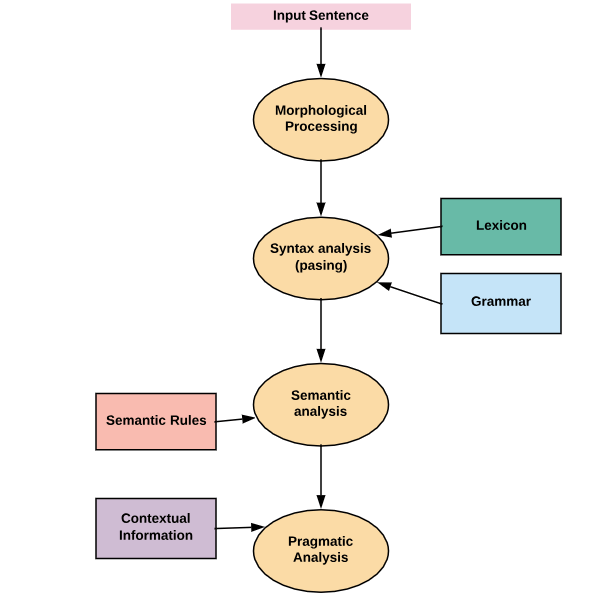
\includegraphics[width =15.5cm]{6.PNG}
		\caption{Component of Natural Language processing }
		\label{ab}
	\end{center}
\end{figure}

Natural Language Understanding is mapping the given input in the natural language into a useful representation.Convert chunks of text into more formal representations such as first-order logic structures that are easier for computer programs to manipulate. Natural language understanding involves the identification of the intended semantic from the multiple possible semantics which can be derived from a natural language expression which usually takes the form of organized notations of natural language concepts. Introduction and creation of language metamodel and ontology are efficient however empirical solutions. An explicit formalization of natural language semantics without confusions with implicit assumptions such as closed-world assumption (CWA) vs. open-world assumption, or subjective Yes/No vs. objective True/False is expected for the construction of a basis of semantics formalization.\\
\subsection{Morphological and Lexical Analysis}
Lexical analysis is a vocabulary that includes its words and expressions. It depicts analyzing, identifying and description of the structure of words. It includes dividing a text into paragraphs, words and the sentences Individual words are analyzed into their components, and nonword tokens such as punctuations are separated from the words.\\Separate words into individual morphemes and identify the class of the morphemes. The difficulty of this task depends greatly on the complexity of the morphology (i.e. the structure of words) of the language being considered. English has fairly simple morphology, especially inflectional morphology, and thus it is often possible to ignore this task entirely and simply model all possible forms of a word (e.g. "open, opens, opened, opening") as separate words. In languages such as Turkish or Meitei, a highly agglutinated Indian language, however, such an approach is not possible, as each dictionary entry has thousands of possible word forms.
\subsection{Semantic Analysis}
Semantic Analysis is a structure created by the syntactic analyzer which assigns meanings. This component transfers linear sequences of words into structures. It shows how the words are associated with each other.One among them is Named entity recognition (NER). Given a stream of text, determine which items in the text map to proper names, such as people or places, and what the type of each such name is (e.g. person, location, organization). Although capitalization can aid in recognizing named entities in languages such as English, this information cannot aid in determining the type of named entity, and in any case is often inaccurate or insufficient. For example, the first letter of a sentence is also capitalized, and named entities often span several words, only some of which are capitalized. Furthermore, many other languages in non-Western scripts (e.g. Chinese or Arabic) do not have any capitalization at all, and even languages with capitalization may not consistently use it to distinguish names. For example, German capitalizes all nouns, regardless of whether they are names, and French and Spanish do not capitalize names that serve as adjectives.\\Semantics focuses only on the literal meaning of words, phrases, and sentences. This only abstracts the dictionary meaning or the real meaning from the given context. The structures assigned by the syntactic analyzer always have assigned meaning\\E.g.. "colorless green idea." This would be rejected by the Symantec analysis as colorless Here; green doesn't make any sense.
\subsection{Pragmatic Analysis}
Pragmatic Analysis deals with the overall communicative and social content and its effect on interpretation. It means abstracting or deriving the meaningful use of language in situations. In this analysis, the main focus always on what was said in reinterpreted on what is meant.\\Pragmatic analysis helps users to discover this intended effect by applying a set of rules that characterize cooperative dialogues.E.g., "close the window?" should be interpreted as a request instead of an order.
\subsection{Syntax analysis}
The words are commonly accepted as being the smallest units of syntax. The syntax refers to the principles and rules that govern the sentence structure of any individual languages.Syntax focus about the proper ordering of words which can affect its meaning. This involves analysis of the words in a sentence by following the grammatical structure of the sentence. The words are transformed into the structure to show hows the word are related to each other.\\One among this is parsing.Determine the parse tree (grammatical analysis) of a given sentence. The grammar for natural languages is ambiguous and typical sentences have multiple possible analyses. In fact, perhaps surprisingly, for a typical sentence there may be thousands of potential parses (most of which will seem completely nonsensical to a human). There are two primary types of parsing, Dependency Parsing and Constituency Parsing. Dependency Parsing focuses on the relationships between words in a sentence (marking things like Primary Objects and predicates), whereas Constituency Parsing focuses on building out the Parse Tree using a Probabilistic Context-Free Grammar (PCFG). See also: Stochastic grammar.
\subsection{Discourse Integration}
It means a sense of the context. The meaning of any single sentence which depends upon that sentences. It also considers the meaning of the following sentence.\\ One among this is Coreference resolution. Given a sentence or larger chunk of text, determine which words ("mentions") refer to the same objects ("entities"). Anaphora resolution is a specific example of this task, and is specifically concerned with matching up pronouns with the nouns or names to which they refer. The more general task of coreference resolution also includes identifying so-called "bridging relationships" involving referring expressions. For example, in a sentence such as "He entered John's house through the front door", "the front door" is a referring expression and the bridging relationship to be identified is the fact that the door being referred to is the front door of John's house (rather than of some other structure that might also be referred to).For example, the word "that" in the sentence "He wanted that" depends upon the prior discourse context.
\section{Architecture of the components of a Conversational Agent}
Approaches to computational architectures of conversa-tional agents vary a great deal with respect to the underly-ing practical requirements, with no agreement betweenresearchers on the most productive approach. This architecture contains sixmodules, each of which corresponds to a certain cognitiveaspect underlying the human language processing system.The speech recognition and natural language understandingmodules extract meaning from the user’s input. The dialo-gue management module controls the dialogue flow. Itaccepts interpreted dialogue acts as input, interacts withexternal knowledge resources (e.g. a task managementcomponent), decides on which dialogue acts should be gen-erated, formulates their meaning, and so on. The naturallanguage generation and speech synthesis components mapfrom meaning to speech. This architecture is rather general,that is, not based on particular requirements. It encapsulatesthe common foundation of different conversational agents,and can be adapted to various conversational scenarios.\\At the other end of the scale, there are a number ofmore elaborate architectures in terms of an increasednumber of modules that implement additional functionalrequirements (e.g. emotion recognition, multimodal inter-action, etc.). The requirements on such architectures arisefrom particular scenarios of use. The advantage of thesearchitectures is that they are based on (more or less) well-defined requirements. The disadvantage is that they arenot really applicable to other scenarios. The trade-offbetween the two ends of the spectrum is apparent, andresearchers tend – for obvious practical reasons – to focuson scenario-specific design.However, it is important to emphasize that speech rec-ognition modules are usually architecture-agnostic all overthis scale. In other words, the research question of speechrecognition is usually considered outside of an architecturalcontext. The researchers take into account dimensions ofvariation in speech recognition tasks such as vocabularysize, fluency of speech, variation in channel and noise, andspeaker-class characteristics.

\begin{figure}[h]
	\begin{center}
		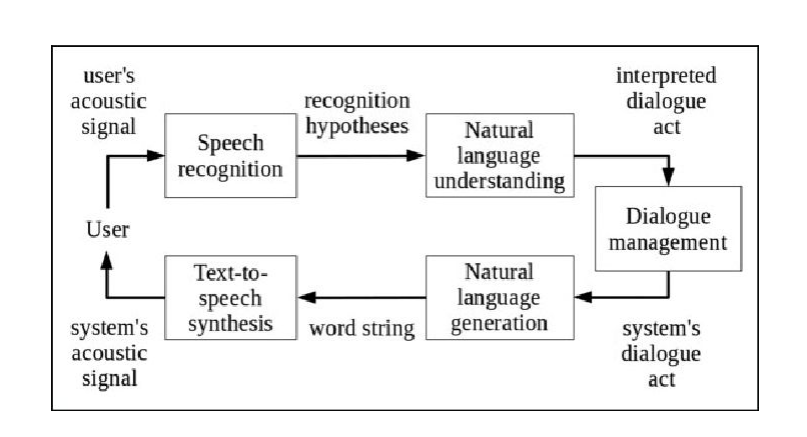
\includegraphics[width =10cm]{7.PNG}
		\caption{Architecture of the components of a Conversational Agent}
		\label{ab}
	\end{center}
\end{figure}


\chapter{CONCLUSION}
Elderly people constitute a significant percentage of the population all over the world. The aim of the study is to explore needs of patients with cognitive deficits and understand the need to help in patient’s daily activities.This paper reports an ongoing research project of for elder people. The core of this research is to apply intelligent techniques to meet particular needs of cognitive deficits patients and assess interplay adjustments based totally on his or her behavior in diverse disease stages.The aim of the study is to explore needs of patients with cognitive deficits and understand the need to help in patient’s daily activities. 















%
%
%
% ***   Creating Bibliography   ***
%
% Do not delete the following two lines
%
\clearpage
\addcontentsline{toc}{chapter}{\quad BIBLIOGRAPHY}
%
%   The markups for creating the bibliography 
%   begins here. Do not change the two lines 
%   "\begin{thebibliography}{99}" and 
%   "\end{thebibliography}".
%   One sample bibliography item is included. 
%   Each new item is to be preceded by
%   "\bibitem{}".
%   Add additional items if there are any.
%   Bibliography styles:
%   Titles of books   : Italics  {use {\em Title} )
%   URLs of websites  : Type-writer (use {\tt Title} )
%   Titles of papers  : In double quotes (use ``Title")
%
\begin{thebibliography}{99}
%
\bibitem{ref1}
 Lee AY (August 2011). "Vascular dementia". Chonnam Medical Journal.

\bibitem{ref2}
Cerejeira J, Lagarto L, Mukaetova-Ladinska EB (2012). "Behavioral and psychological symptoms of dementia". Frontiers in Neurology. 3: 73.


\bibitem{ref3}
Calleo J, Stanley M (2008). "Anxiety Disorders in Later Life Differentiated Diagnosis and Treatment Strategies". Psychiatric Times. 25 (8).  from the original on 2009-09-04.

\bibitem{ref4}
Hugo J, Ganguli M (August 2014). "Dementia and cognitive impairment: epidemiology, diagnosis, and treatment". Clinics in Geriatric Medicine. 30 (3): 421–42.
\bibitem{ref5}
J. Zhou and G. Salvendy, “Human aspects of IT for the aged population: Design for everyday life: First International Conference, ITAP 2015 held as part of HCI International 2015 Los Angeles, CA, USA, August 2–7, 2015 proceedings, part II,” Lect. Notes Comput. Sci. (including Subser. Lect. Notes Artif. Intell. Lect. Notes Bioinformatics), vol. 9194, pp. 465–475, 2015. 
\bibitem{ref6}
Z. Guendil, Z. Lachiri, and C. Maaoui, “Computational framework for emotional VAD prediction using regularized Extreme Learning Machine,” Int. J. Multimed. Inf. Retr., vol. 6, no. 3, pp. 251– 261, 2017 
\bibitem{ref7}
Do Kook Choe and Eugene Charniak (EMNLP 2016). https://aclanthology.coli.uni-saarland.de/papers/D16-1257/d16-1257 Parsing as Language Modeling


%
\end{thebibliography}
%
%   ***   Creating Index   ***
%
%   To add a particular word, say abcxyz, to index write 
%   the command \index{abcxyz} near the word where it 
%   first appears in the text. Include all technical 
%   sounding words in the index. 
%   Do not delete the following three lines.
%
%\clearpage
%\addcontentsline{toc}{chapter}{\quad INDEX}
%\printindex
%
\clearpage
\addcontentsline{toc}{chapter}{\quad APPENDIX}
\chapter*{\centering{APPENDIX}}
%%%%%%%%%%%%%%%%%%%%%%%%%%%%%%%%%%%%%
%%                          
%%		APPENDIX
%%    if u have pgms make that a pdf & add it here, like the data sheets
%%
%%    If you need to give an Intro to the Appendix
%%                                 Otherwise Delete it . . . 
%%
%%%%%%%%%%%%%%%%%%%%%%%%%%%%%%%%%%%%%
%%%%%%%%%%%%%%%%%%%%%%%%%%%%%%%%%%%%%

\begin{itemize}
\item Reference Paper of the Seminar-A Proposed Effective Framework for Elderly with Dementia Using Data Mining
\item PPT of the Seminar
\end{itemize}

%%%%%%%%%%%%%%%%%%%%%%%%%%%%%%%%%%%%%
%%%%%%%%%%%%%%%%%%%%%%%%%%%%%%%%%%%%%
%%                      
%%                      For Adding PDF (Data Sheets) for the Appendix
%%
%%%%%%%%%%%%%%%%%%%%%%%%%%%%%%%%%%%%%
%%%%%%%%%%%%%%%%%%%%%%%%%%%%%%%%%%%%%


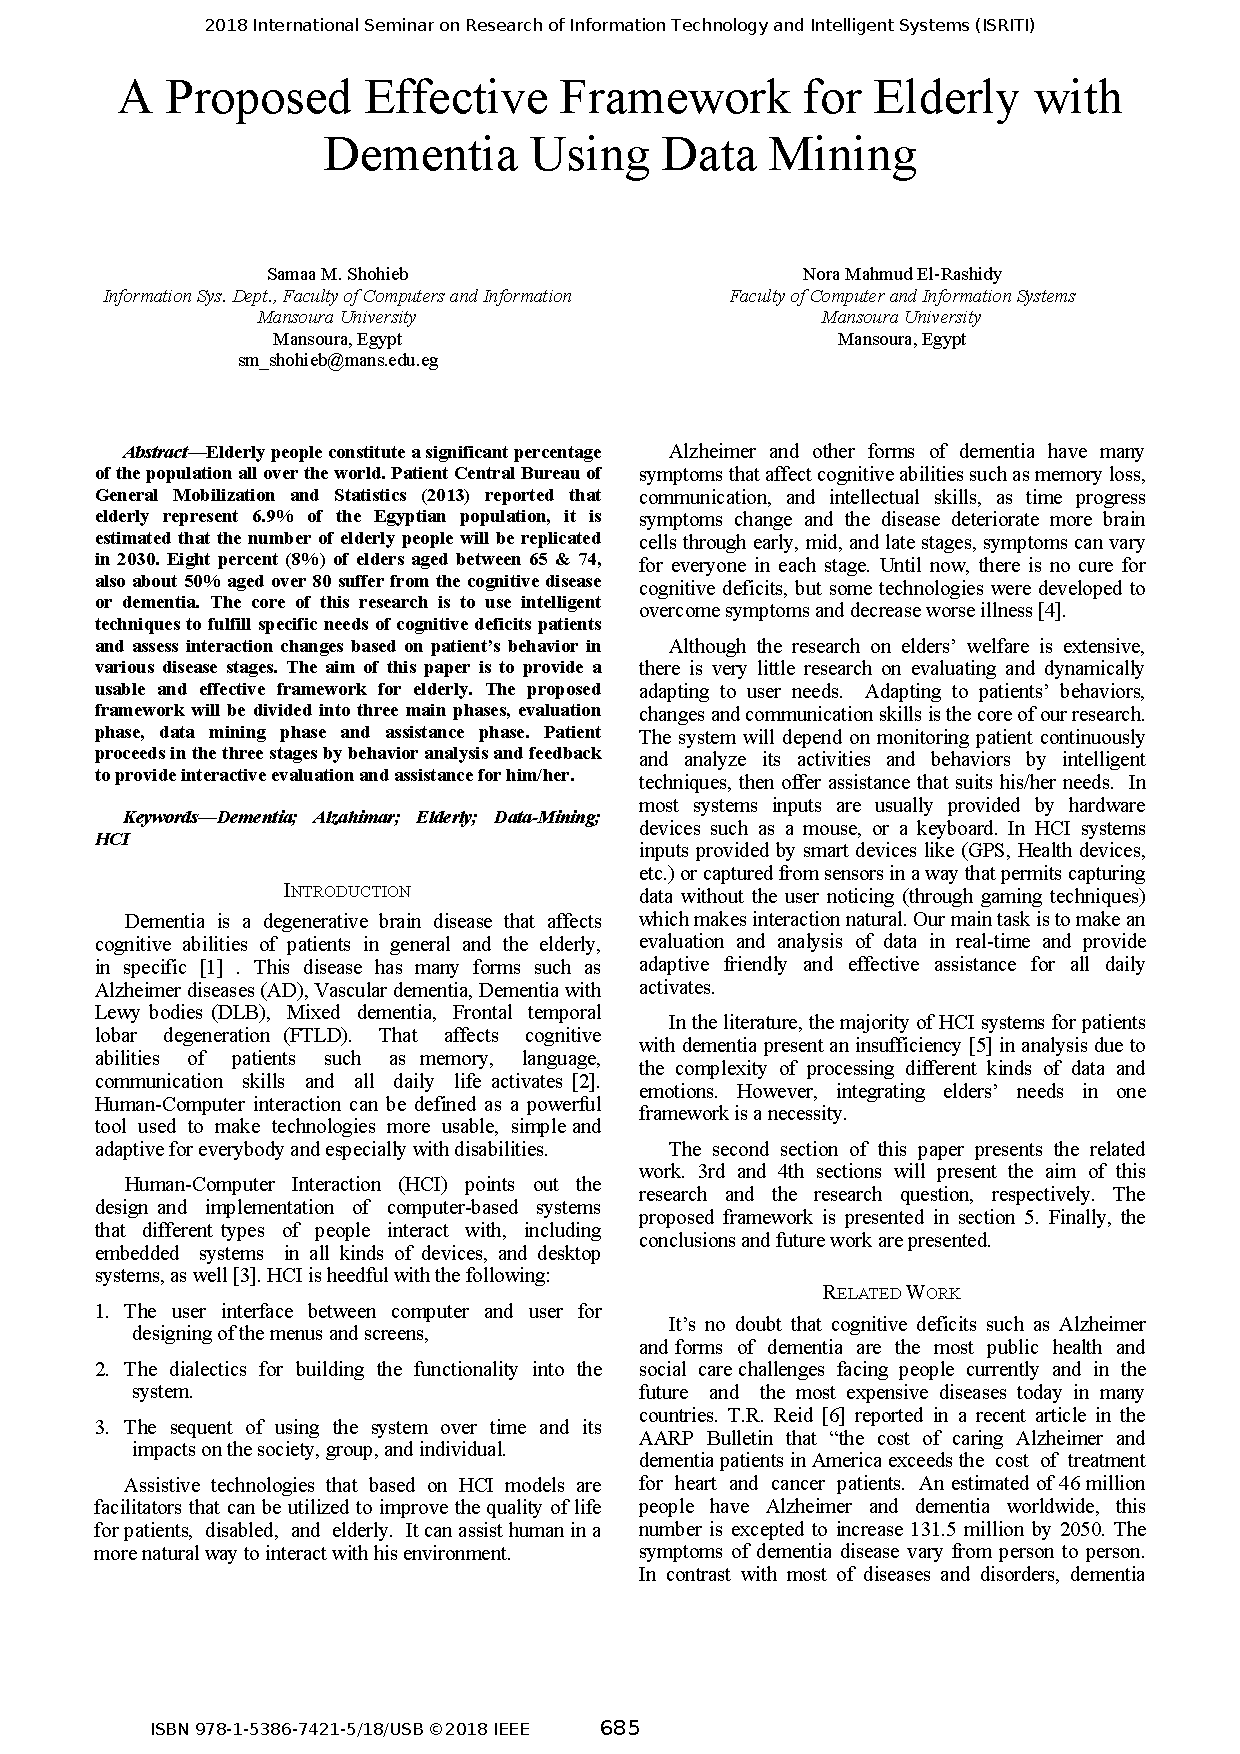
\includepdf[pages=-]{paper.pdf}    % for adding Paper in PDF (same folder)
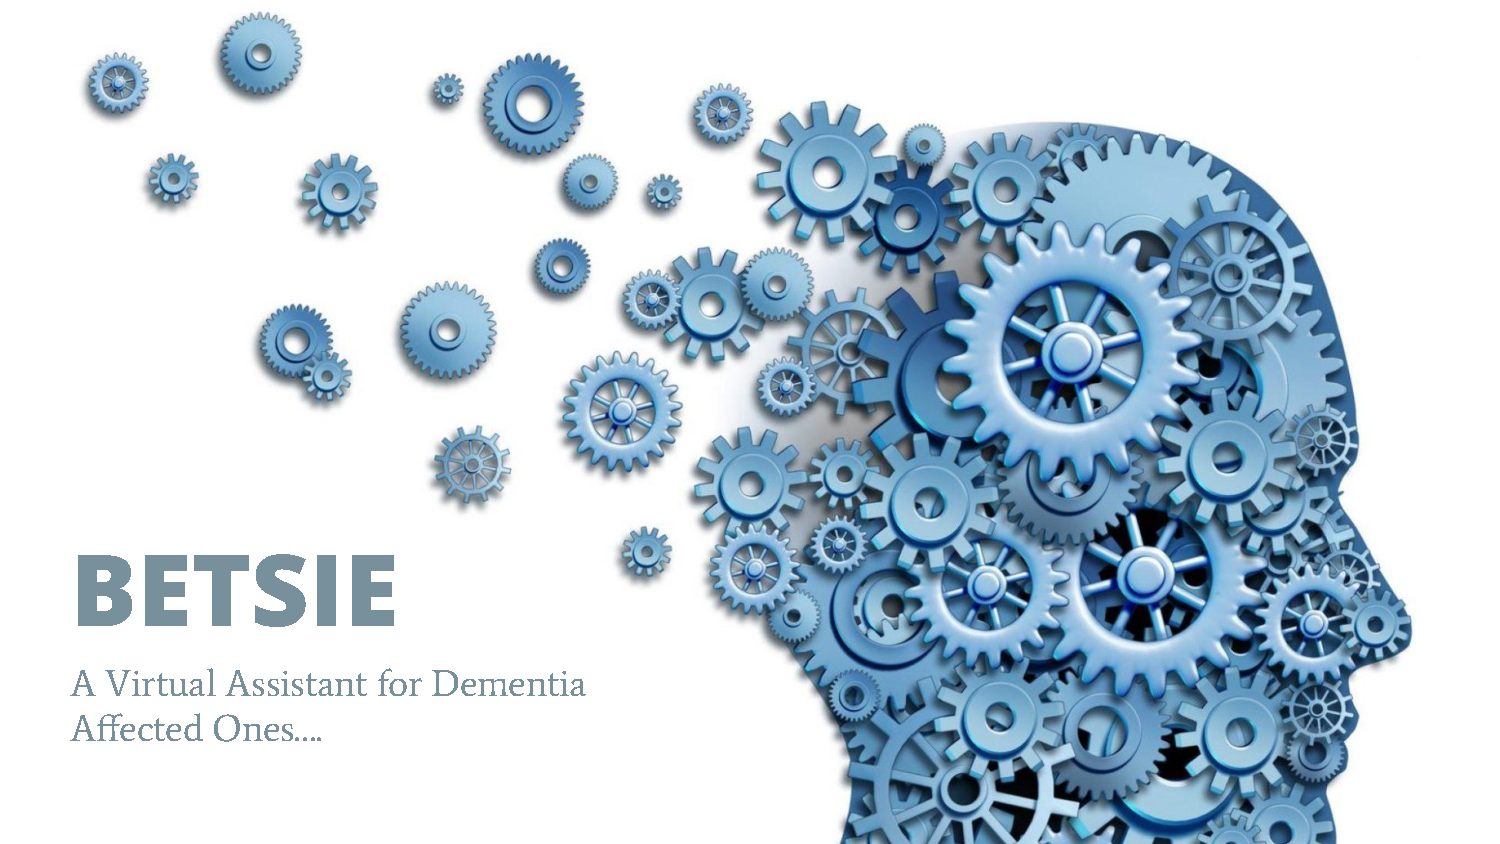
\includepdf[pages=-]{ppt.pdf}    % for adding PPT in PDF in 1 Page 6 Slides


%%%%%%%%%%%%%%%%%%%%%%%%%%%%%%%%%%%%%
%%%%%%%%%%%%%%%%%%%%%%%%%%%%%%%%%%%%%
%%%%%%%%%%%%%%%%%%%%%%%%%%%%%%%%%%%%%
%%%%%%%%%%%%%%%%%%%%%%%%%%%%%%%%%%%%%




%   Printing the last page
%
%%%%%%%%%%%%%%%%%%%%%%%%%%%%%%%%%%%%%
%%%%%%%%%%%%%%%%%%%%%%%%%%%%%%%%%%%%%
%
%   Hi, All
%   Arun Xavier, VAST Thrissur
%
%   for more  Visit my Page - http://arunxeee.blogspot.in/
%
%%%%%%%%%%%%%%%%%%%%%%%%%%%%%%%%%%%%
%%%%%%%%%%%%%%%%%%%%%%%%%%%%%%%%%%%%
%
%
%
%******************************************************
%

%
\end{spacing}
\newpage
\thispagestyle{empty}
\vspace*{\fill}
\begin{flushright}

\includegraphics[width=2.5 cm]{VidyaLogo.JPG}\\[.2 cm]
{\Large \bf \rm  Department of \vdept\ }\\
{\large \rm Vidya Academy of Science \& Technology\\
Thalakkottukara, Thrissur - 680 501\\
({\tt http://www.vidyaacademy.ac.in})}
\end{flushright}

%
%
%
%   ***   The end   ***
%
%
\end{document}


%%%%%%	Any Problems Contact me  @  arunxeee.blogspot.com
%%%%%									aruncx@gmail.com
%%%%%%%%%%%%%%%%
%%%%
%%%%
%%%%%%%%%%%
%%
%
